\documentclass[jkps,preprint,fleqn,showpacs,showkeys]{revtex4}

\usepackage{graphicx}
\usepackage{amssymb}
\usepackage{amsmath}
\usepackage{bm}
\usepackage{lineno}
\usepackage{xspace}
\usepackage{cleveref}
\usepackage {xcolor}

\newcommand{\XGB}{XGBoost}

\begin{document}
\setcounter{page}{0}
\title[]{ MC-based feasibility study of new sampling calorimeter for measuring the $\gamma$ incident angle }

\author{YoungJun \surname{Kim}}
\author{Jung Keun \surname{Ahn}}
\affiliation{Department of Physics, Korea University, Seoul 02841}
\author{Junlee \surname{Kim}}
\email{junlee.kim@cern.ch}
\author{Eun-Joo \surname{Kim}}
\email{ejkim@jbnu.ac.kr}
\affiliation{Department of Physics education, Jeonbuk National University, Jeonju 54896}
\author{GeiYoub  \surname{Lim}}
\affiliation{IPNS/KEK Tsukuba, Japan 305-0801}

%\date[]{Received 6 August 2007}

\begin{abstract}
We present studies on the detector configuration to measure the incident angle of the $\gamma$ with energies ranging from hundred MeV to few GeV using a new sampling calorimeter. The sampling calorimeter consists of alternating 1-mm-thick lead plates producing the electromagnetic (EM) shower and strips of 5-mm-thick plastic scintillators measuring the energy deposit by the shower particles. The strips are arranged along the alternating horizontal and vertical directions to measure the transverse profile by combining both directions at a given longitudinal position. In this paper, we used the GEANT4 to simulate energy deposit to the individual strips of the calorimeter, and the $\XGB$ to reconstruct the incident angle from energy deposits. 

The angular resolution weakly depends on the width of the strips up to 15 mm and becomes worse with the increasing width. It is found that the incident angle is reconstructed with the compatible angular resolution using front 5 radiation length (5$X_{0}$) of the detector. The resolution does not depend on the incident angle up to 30 degrees, and largely depends on the incident energy, which can be expressed as 0.2+1.1$/ \sqrt{E_\gamma}$.

\end{abstract}

%\pacs{68.37.Ef, 82.20.-w, 68.43.-h}
%\keywords{String shoving, Collectivity, $pp$ collision}
\maketitle

\section{Motivation}
\label{sec:mot}
The EM calorimeter has played an important role in experimental studies for the nuclear and particle physics. Various materials have been developed for better energy and timing resolution so far~\cite{Calorimeter}. On the other side, the sampling calorimeter becomes popular in the large-scale high energy experiment mainly due to its cost-effectiveness. The sampling calorimeter consists of alternating passive converters that generate the EM shower and active counters that measure the energy deposit. Since the energy deposit in the passive convert is not measured, the fluctuation of energy deposits in the converter and the counter, called sampling fluctuation, determines the energy resolution of the calorimeter. The sampling fluctuation can be optimized by combining the converter and the counter with a specific portion. A 5-m-long cylindrical calorimeter made of alternating lead plates and plastic scintillating plates is an example of the sampling calorimeter~\cite{E391a_barrel}.

The layer structure of the sampling calorimeter allow one to measure the individual profile of the shower along the beam direction, and the incident angle can be estimated by correlating energy deposits on neighboring layers. The measurement of the incident angle largely benefits the background rejection. Of particular, The incident angle will be an important tool for the KOTO experiment~\cite{KOTOproposal}.

Since the EM shower is evolving via stochastic processes, the incident angle would be reconstructed with a certain angular resolution. Energy deposits from random processes are used to reconstruct the incident angle with the machine learning, which provides better angular resolution. The evolution of the EM shower is generated with the GEANT4, and the $\XGB$ was used to reconstruct the incident angle.

In sec~\ref{sec:ems}, generic explanation of the EM shower and its evolution are described. We describe the reconstruction and angular resolution of the sampling calorimeter in sec~\ref{sec:res}. We summarize the study in sec~\ref{sec:sum}.

\section{ELECTROMAGNETIC SHOWER}
\label{sec:ems}

\begin{figure}[!hbt]
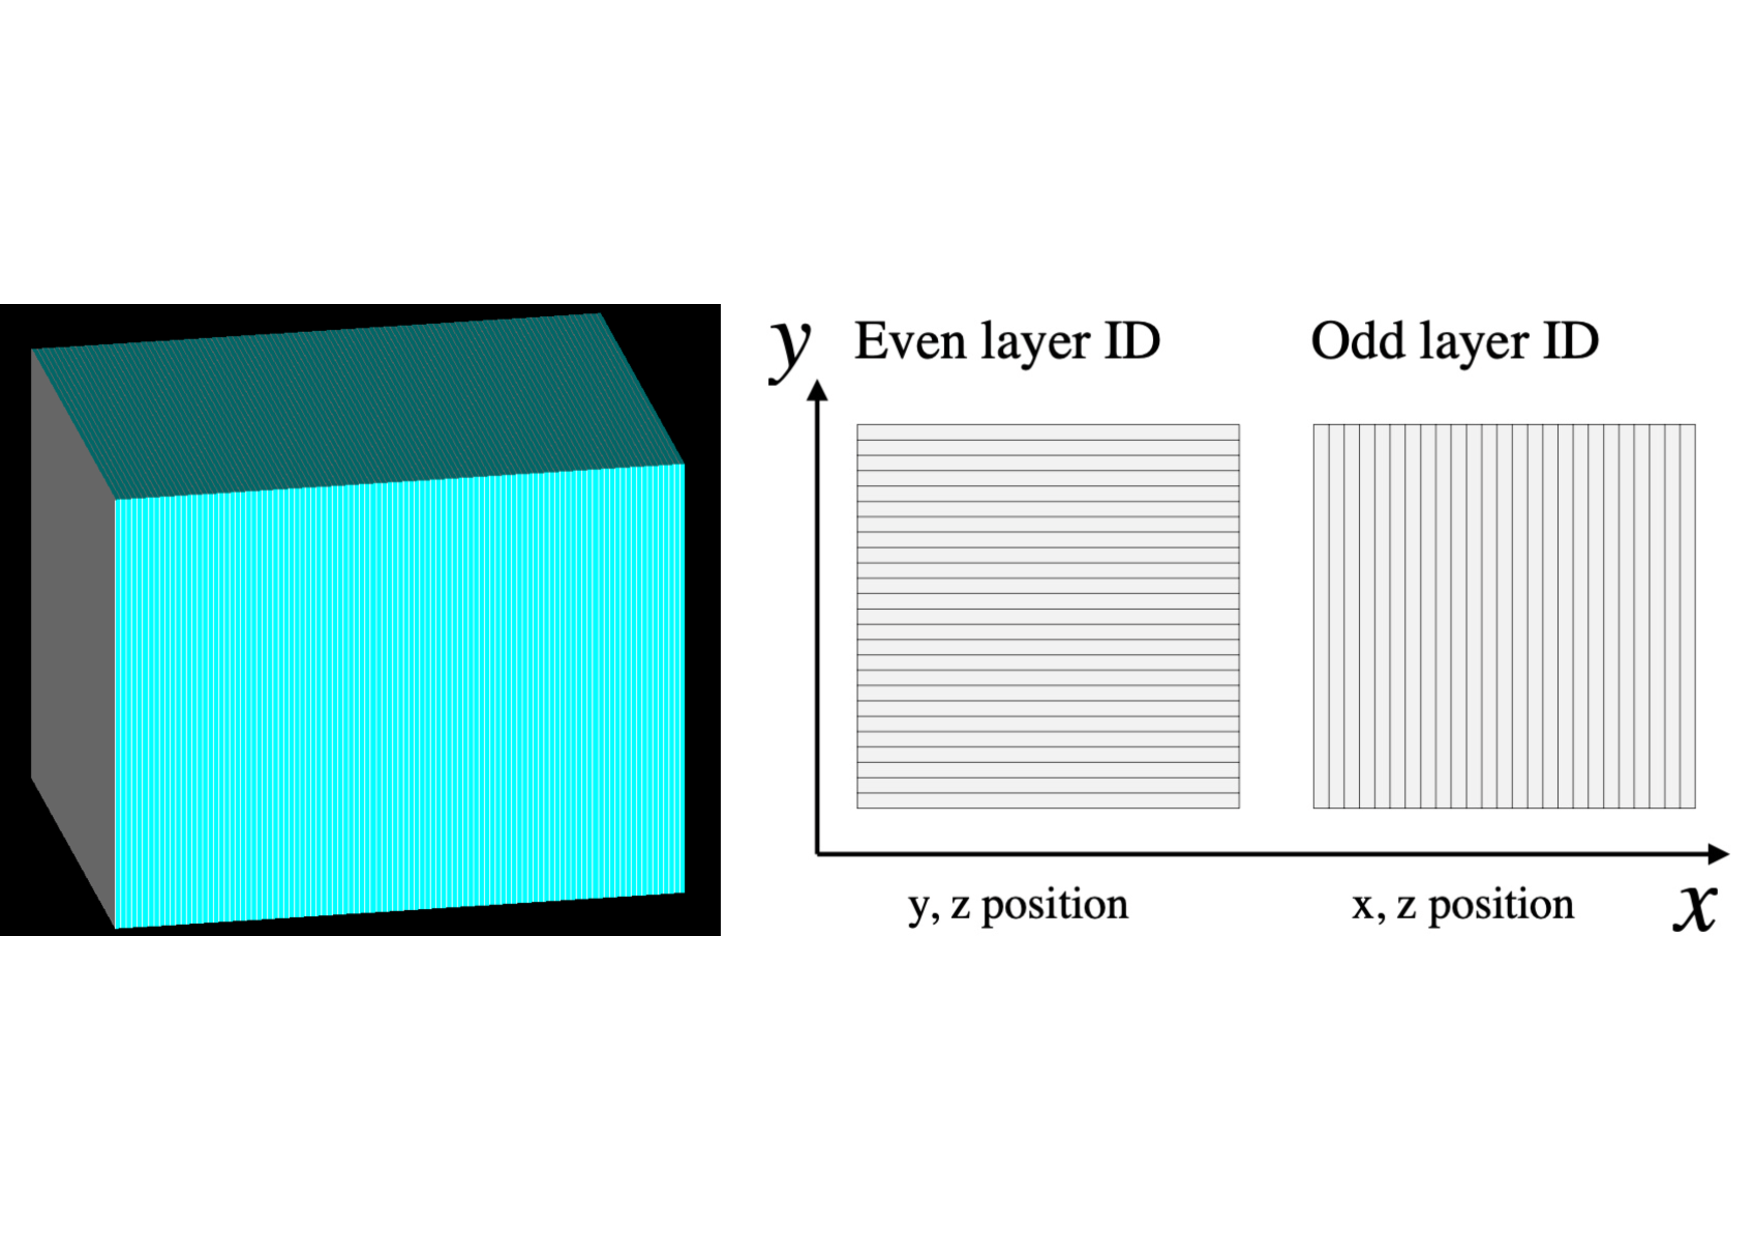
\includegraphics[width=0.85\textwidth]{figures/Sec2/Prototype_samplingcal.pdf}
\caption{ \textcolor{red}{plots should be updated} Schematic view of the sampling calorimeter. It consists of 105 alternating lead plates and scintillator strips. Each scintillator layer consists of 35 scintillator strips. The cross section of each 1-mm-thick lead plate is 525 mm $\times$ 525 mm. The cross section of each 5-mm-tihck scintillator strip is 525 mm $\times$ 15 mm. }
\label{fig:det_conf}
\end{figure}

The sampling calorimeter was designed as alternating 1-mm-thick lead plates for passive converters and 5-mm-thick strips of the plastic scintillator for active counters. Strips are alternatively aligned along $x$ and $y$ direction as shown in Fig.~\ref{fig:det_conf}. The cross section of the lead plate and the scintillator is 525 mm $\times$ 525 mm and 15 mm $\times$ 525 mm, respectively. The material for the scintillator strip is polyvinyltoluene. The total number of alternating layers is 105, which corresponds to 20$X_{0}$ to make it possible to absorb whole products from the EM shower ranging from 100 MeV to few GeV energy.

\begin{figure}[!hbt]
%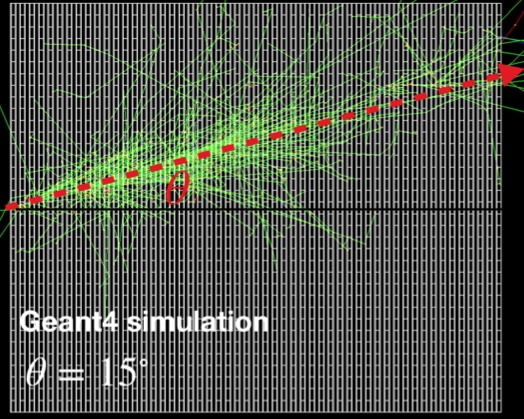
\includegraphics[width=0.45\textwidth]{figures/EventDisplay.jpg}
%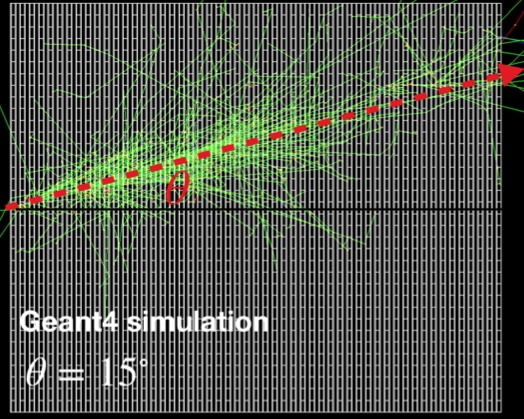
\includegraphics[width=0.45\textwidth]{figures/EventDisplay.jpg}
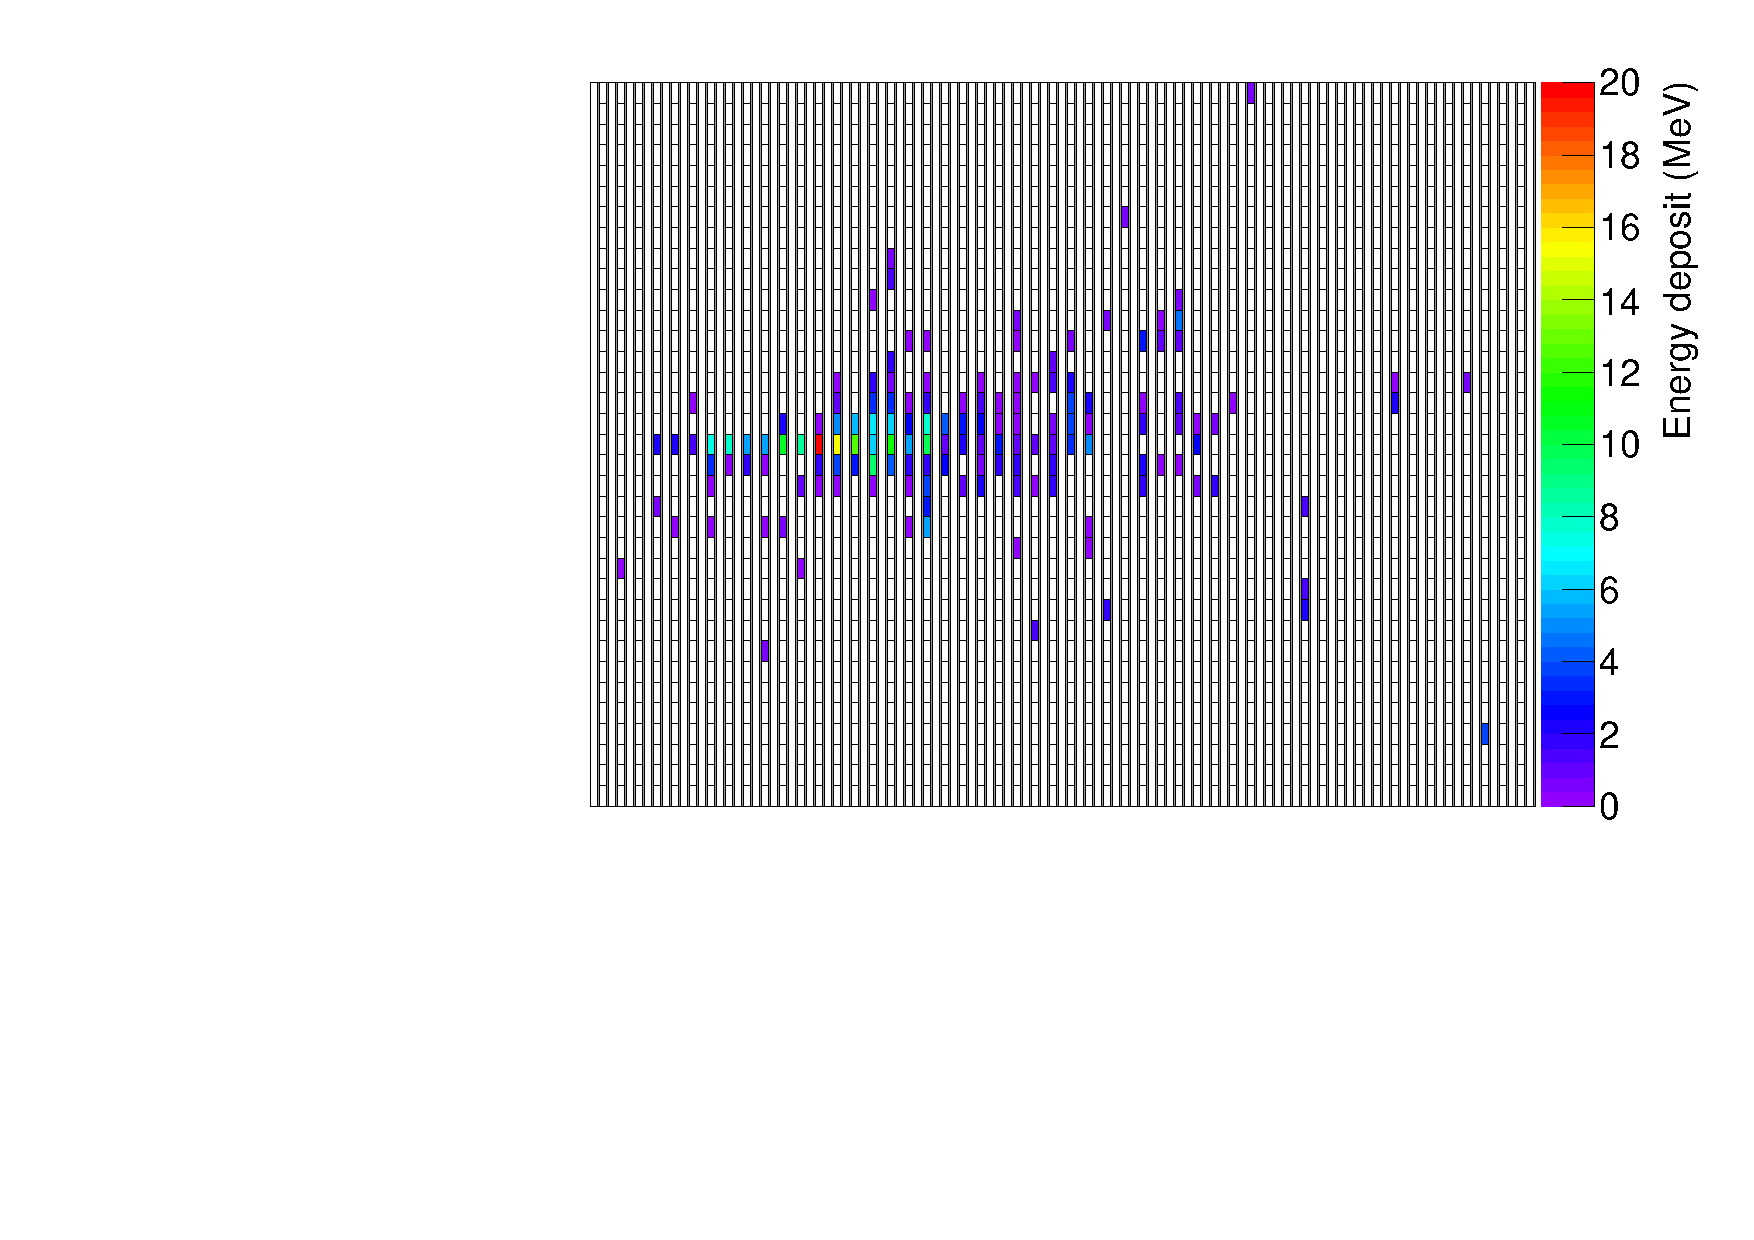
\includegraphics[width=0.48\textwidth]{figures/SingleEventXZHit.pdf}
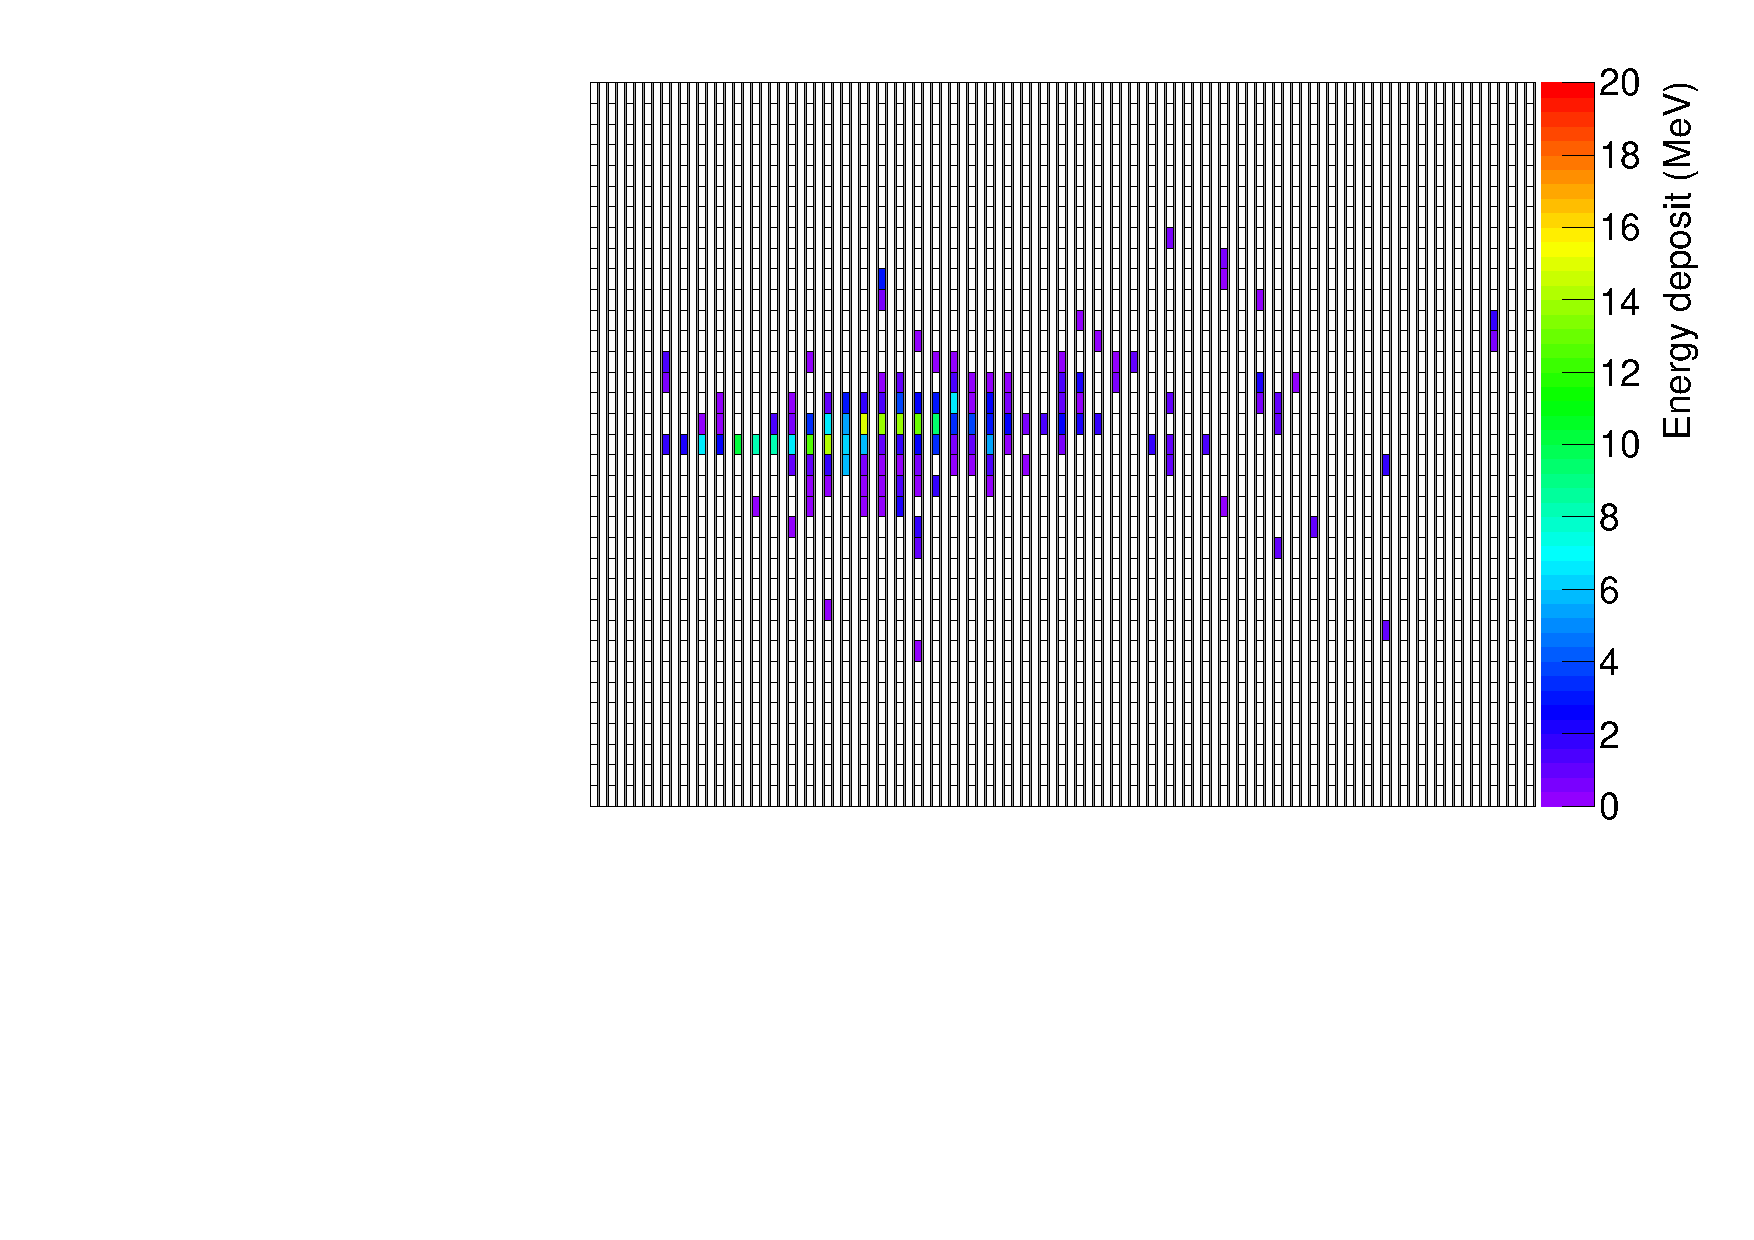
\includegraphics[width=0.48\textwidth]{figures/SingleEventYZHit.pdf}
\caption{ An event display of the energy deposit to each scintillator strip in the $x$--$z$ plane (left) and the $y$--$z$ plane (right) for the 1~GeV $\gamma$ perpendicularly entering to the detector ($\theta=$~0).}
\label{fig:Evt_Dis}
\end{figure}

The interaction of incident $\gamma$ with the detector was simulated using the GEANT4 (ver. 4.10.06) with the standard EM sub-packages~\cite{GEANT4}. The surface of the detector is defined as $z=$~0, and the $\gamma$ starts to interact with the detector. the incident angle of the $\gamma$ is defined as the polar angle ($\theta$) along the $z$ direction, where $\theta = 0$ case denotes that the $\gamma$ perpendicularly enters into the detector surface. Figure~\ref{fig:Evt_Dis} shows the event display illustrating the energy deposit on the each scintillator strip in both of $x$--$z$ and $y$--$z$ planes for the 1~GeV~$\gamma$ with $\theta = 0$.

%\begin{figure}[!hbt]
%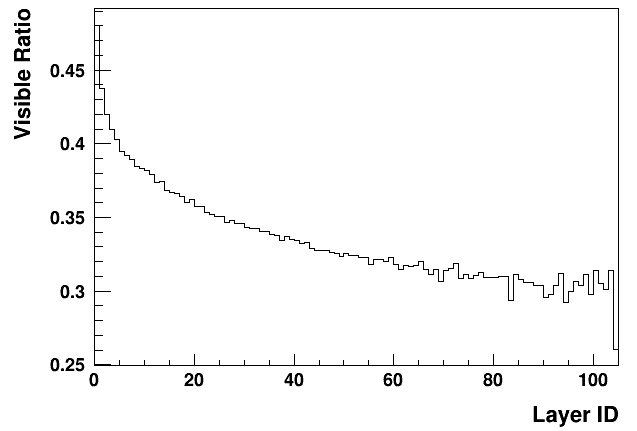
\includegraphics[width=0.48\textwidth]{figures/LayerVisibleRatio.jpg}
%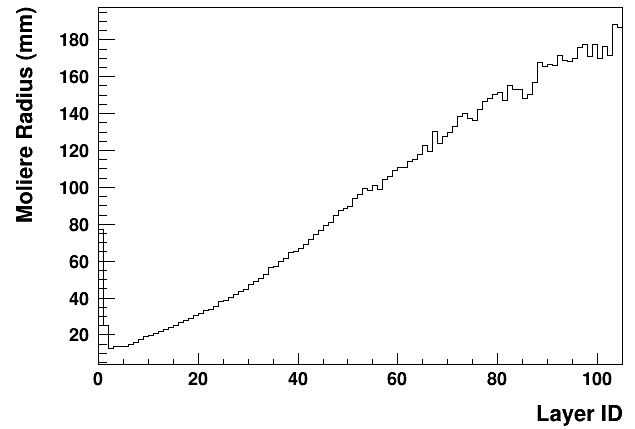
\includegraphics[width=0.48\textwidth]{figures/Moliere_layer.jpg}
%\caption{  \textcolor{red}{plots should be updated} Sampling fraction (left) and Moliere radius (right) from 1 GeV %$\gamma$ events ($\theta=0$) for each layer}
%\label{fig:sc_prop}
%\end{figure}

%Figure~\ref{fig:sc_prop} shows the sampling fraction and the Moliere radius~\cite{PDG} for each layer with 1~GeV $\gamma$. In this paper, Moliere radius is defined as the distance including 90\% of (deposited) energy from the center of energy. The visible ratio (Moliere radius) decreases (increases) with increasing layer ID. It is, therefore, estimated to have better energy resolution and position separation with front layers. Note that the very front few layers are largely affected by secondaries going backward. 

\section{ANGLE RECONSTRUCTION}
\label{sec:res}

The incident angle of the $\gamma$ is reconstructed with the $\XGB$, which is one of the popular machine learning toolkit providing a scalable tree boosting system~\cite{xgboost:2016}. The machine learning is required to be trained. The feature, characteristic of a phenomenon, and the target, output to be predicted, are essential inputs for the training. The machine learning correlates each feature with the corresponding target for different features. Trained machine learning takes measured features and gives the target based on correlations which are made during the training. In this paper, the feature corresponds to energy deposits on each scintillator strip and the target corresponds to the incident angle of the $\gamma$.

If the feature for the training is biased, the prediction of the $\XGB$ would be correspondingly biased as the $\XGB$ reliably believes there are no biases in all features given by a user. To minimize this, the incident angle is uniformly generated in the range 0 to 50 degrees for incident polar angle ($\theta$) and 0 to 360 degrees for incident azimuthal angle ($\varphi$), which makes the $\XGB$ train all features we are interested in. The number of samples for the training is $2\times10^5$ considering computing resources. To test the reconstruction of the incident angle, the incident angle is generated with the fixed $\theta$. Note that the incident energy is known.

\begin{figure}[!hbt]
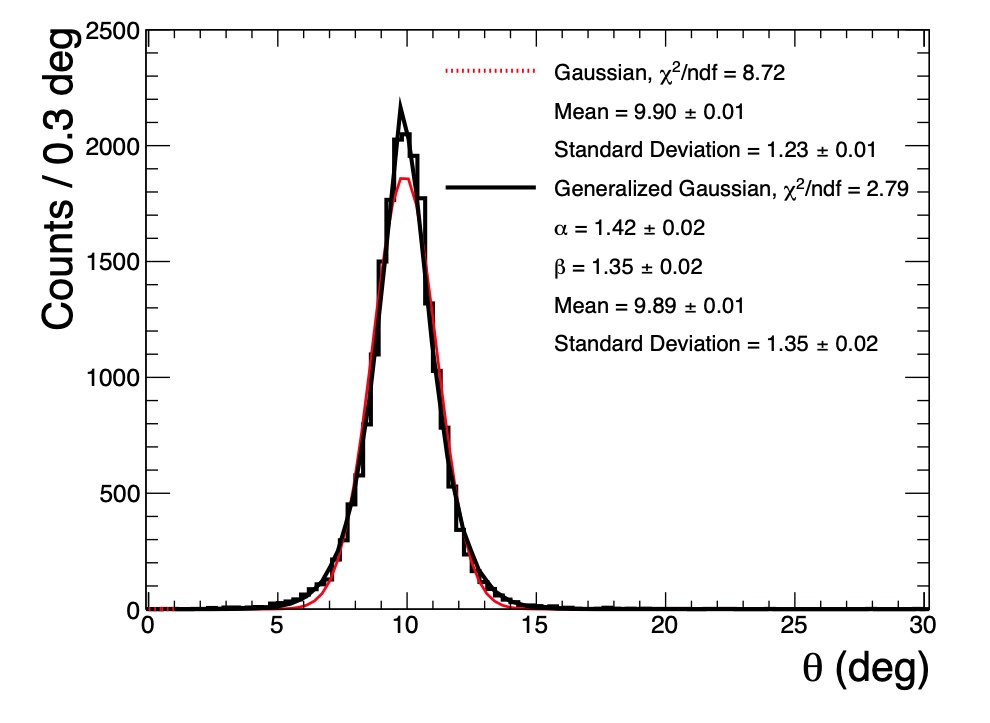
\includegraphics[width=0.7\textwidth]{figures/GG_fit.jpg}
\caption{ Reconstructed $\theta$ distribution for $\theta=$~10~deg events. The distribution is fitted with the Gaussian function and the Generalized Gaussian function. The Generalized Gaussian function provides better description for both tails.}
\label{fig:angle_10degree}
\end{figure}

Figure~\ref{fig:angle_10degree} shows reconstructed $\theta$ for 1~GeV $\gamma$ with $\theta=$~10~degrees. The distribution is fitted with the Gaussian function and the Generalized Gaussian (GG) function. GG function provides better description for both tails of the distribution. The GG function can be expressed as
\begin{equation} 
f(x; \mu, \alpha, \beta) = \frac{\beta}{2 \alpha \Gamma(1/\beta)}e^{-(|x-\mu|/\alpha)^\beta}
\end{equation}
The variation of the GG function can be expressed as, then, $\sigma^2 \equiv \alpha^2 \Gamma(3/\beta) / \Gamma(1/\beta)$. The angular resolution of the incident angle reconstruction is defined as $\sigma$.

\begin{figure}[!hbt]
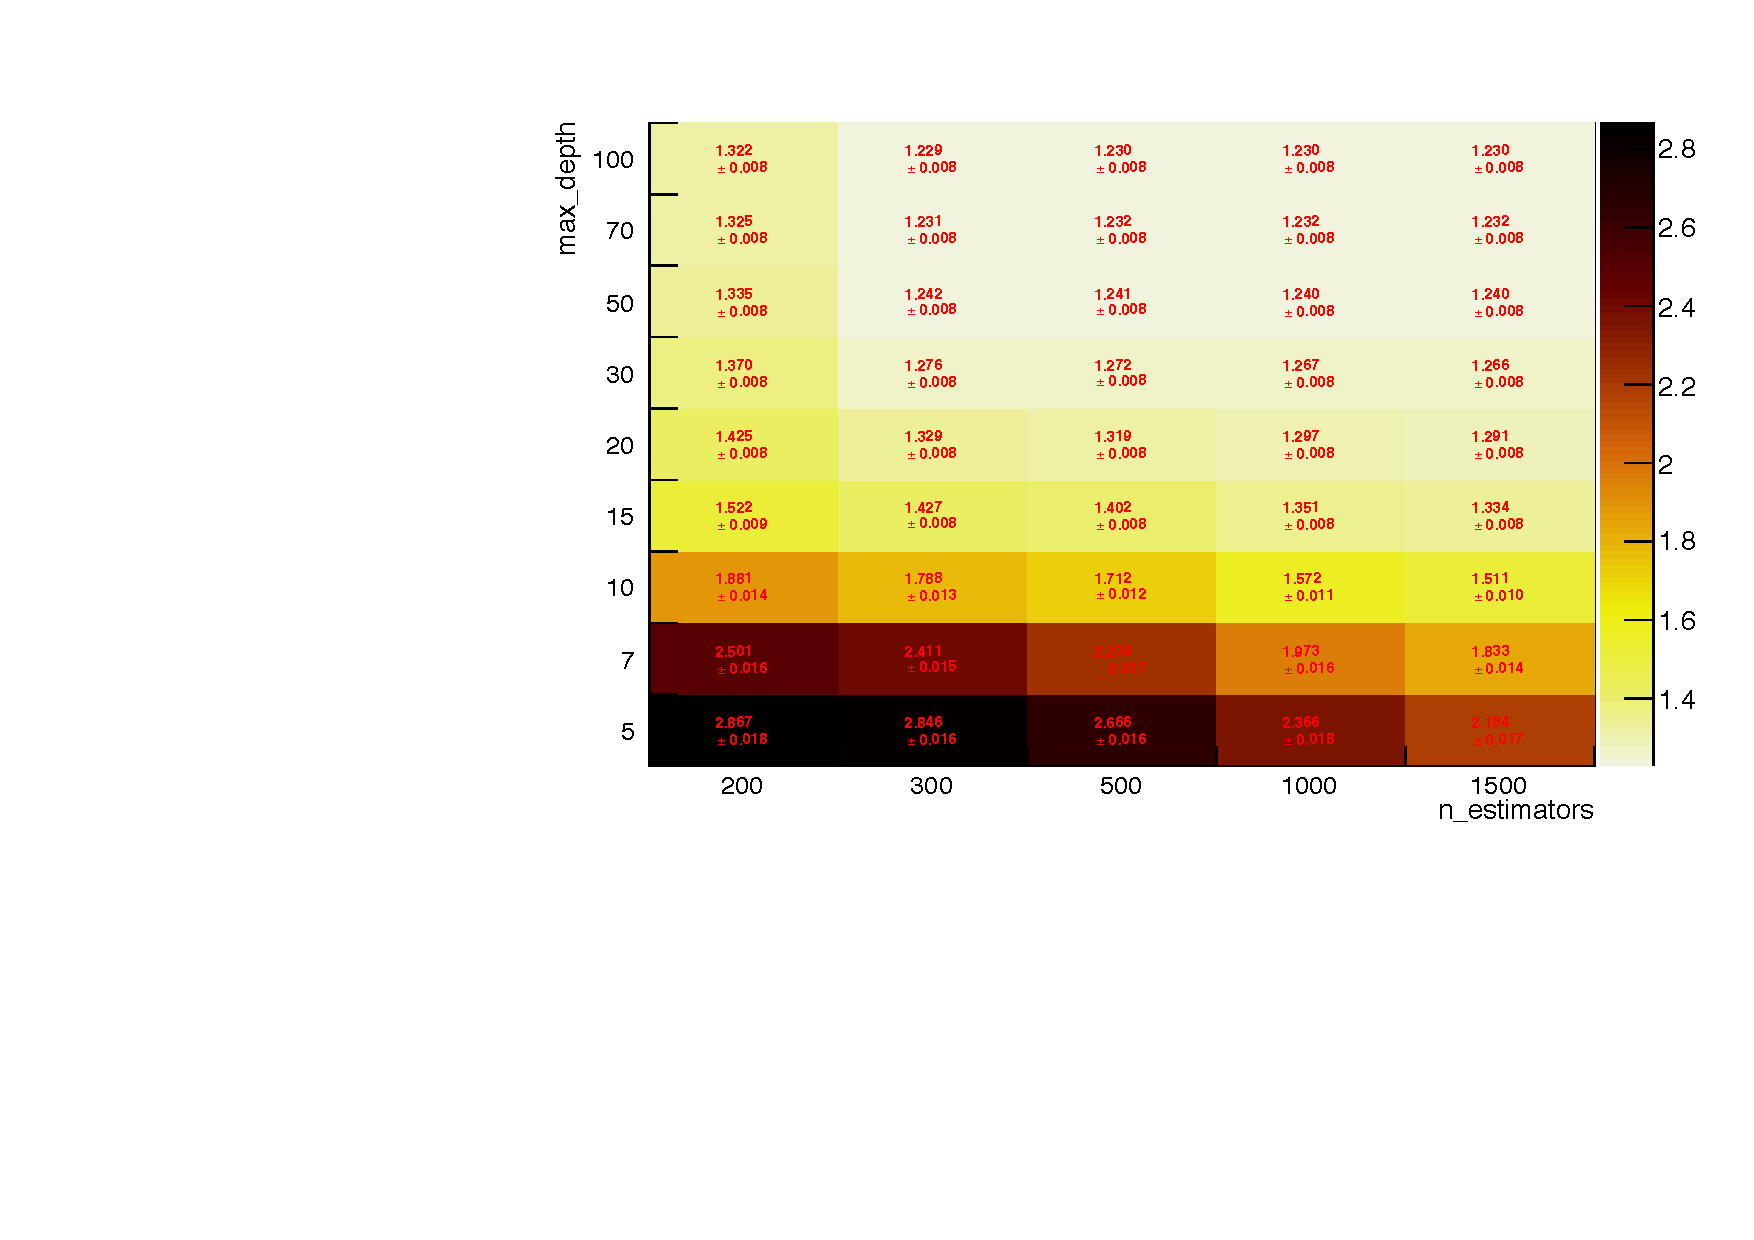
\includegraphics[width=0.89\textwidth]{figures/optimization_plot.pdf}
\caption{The angular resolution for the varying N\_estimators and the varying Max. depth. The best angular resolution is obtained with N\_estimators=300 and Max. depth=100.  }
\label{fig:par_scan}
\end{figure}

As the reconstruction of the incident angle depends on hyperparameters of the $\XGB$, which controls the details of training processes, dedicated tests to optimize the hyperparameter were executed. It is assumed that a set of hyperperameters providing the best angular resolution would be optimized. The test scans the evaluated angular resolution with different hyperparameters. Figure~\ref{fig:par_scan} shows the result of the test for N\_estimators and Max. depth. N\_estimators defines allowed maximal number of decision trees, and the Max. depth defines complexity of the structure of decision trees. The N\_estimators and Max. depth are determined to be 300 and 100, respectively. Similar tests are applied to different hyperparameters, and definitive values for each hyperparameter are shown in Tab~\ref{tab:XgbPar}.
 
\begin{table}[hbt!]
\centering
\caption{Hyperparameters of the $\XGB$}
\begin{tabular}{cccc}
\hline 
Parameter & Function & Default value & Used value \\ \hline 
N\_estimators & The number of decision trees & N.A. & 300 \\  
Max. depth & Possible maximum depth of tree structure & 6 & 100 \\ 
Subsample & Fraction of total data used for a single decision & 1 & 0.8 \\ 
Learning rate & Step length for calculation & 0.3 & 0.02 \\ 
Gamma & Requirement on minimum loss function & 0 & 0 \\ 
\hline
\end{tabular}
\label{tab:XgbPar}
\end{table}

\begin{figure}[!hbt]
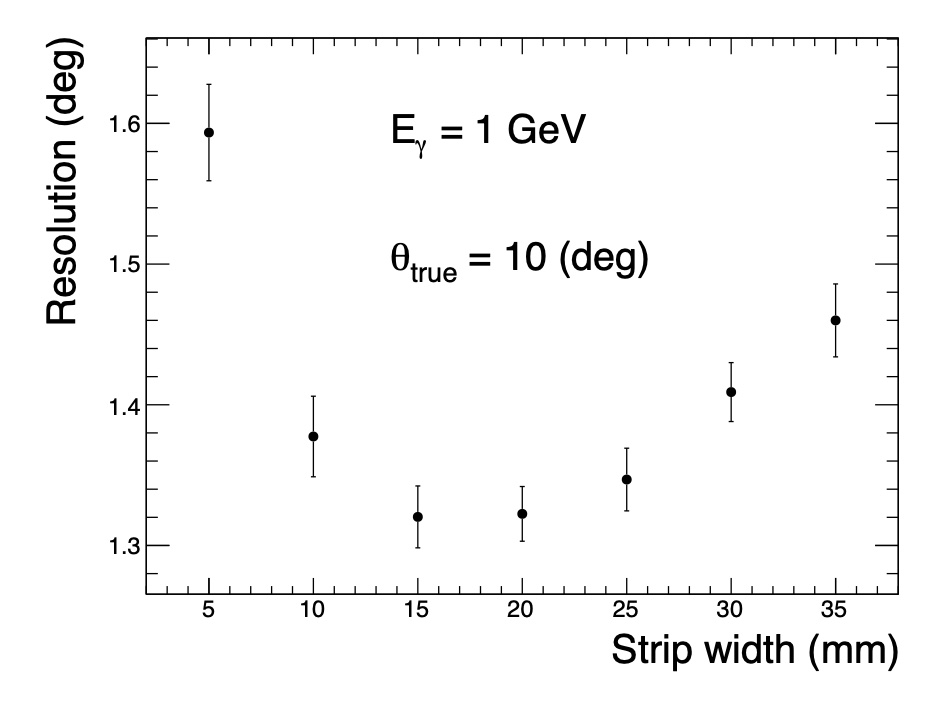
\includegraphics[width=0.58\textwidth]{figures/res_width.jpg}
\caption{ The angular resolution as a function of the scintillator strip width for 1~GeV $\gamma$ with $\theta=$~10~deg. The angular resolution is optimized with 15- to 20-mm-wide strips.}
\label{fig:angle_reco_width}
\end{figure}

The angular resolution was evaluated with the width of scintillator strips varying from 5 mm to 35 mm. Figure~\ref{fig:angle_reco_width} shows the angular resolution as a function of the width. 15-mm-wide strips provide the best angular resolution. The width longer than 15 mm suffers from the dilution of the EM shower, resulting in worse resolution. On the other hand, the width shorter than 15 mm results in larger size of features, which causes a negative influence on the machine learning. Dedicated study is described in fig~\ref{fig:angle_reco_width}.

\begin{figure}[!hbt]
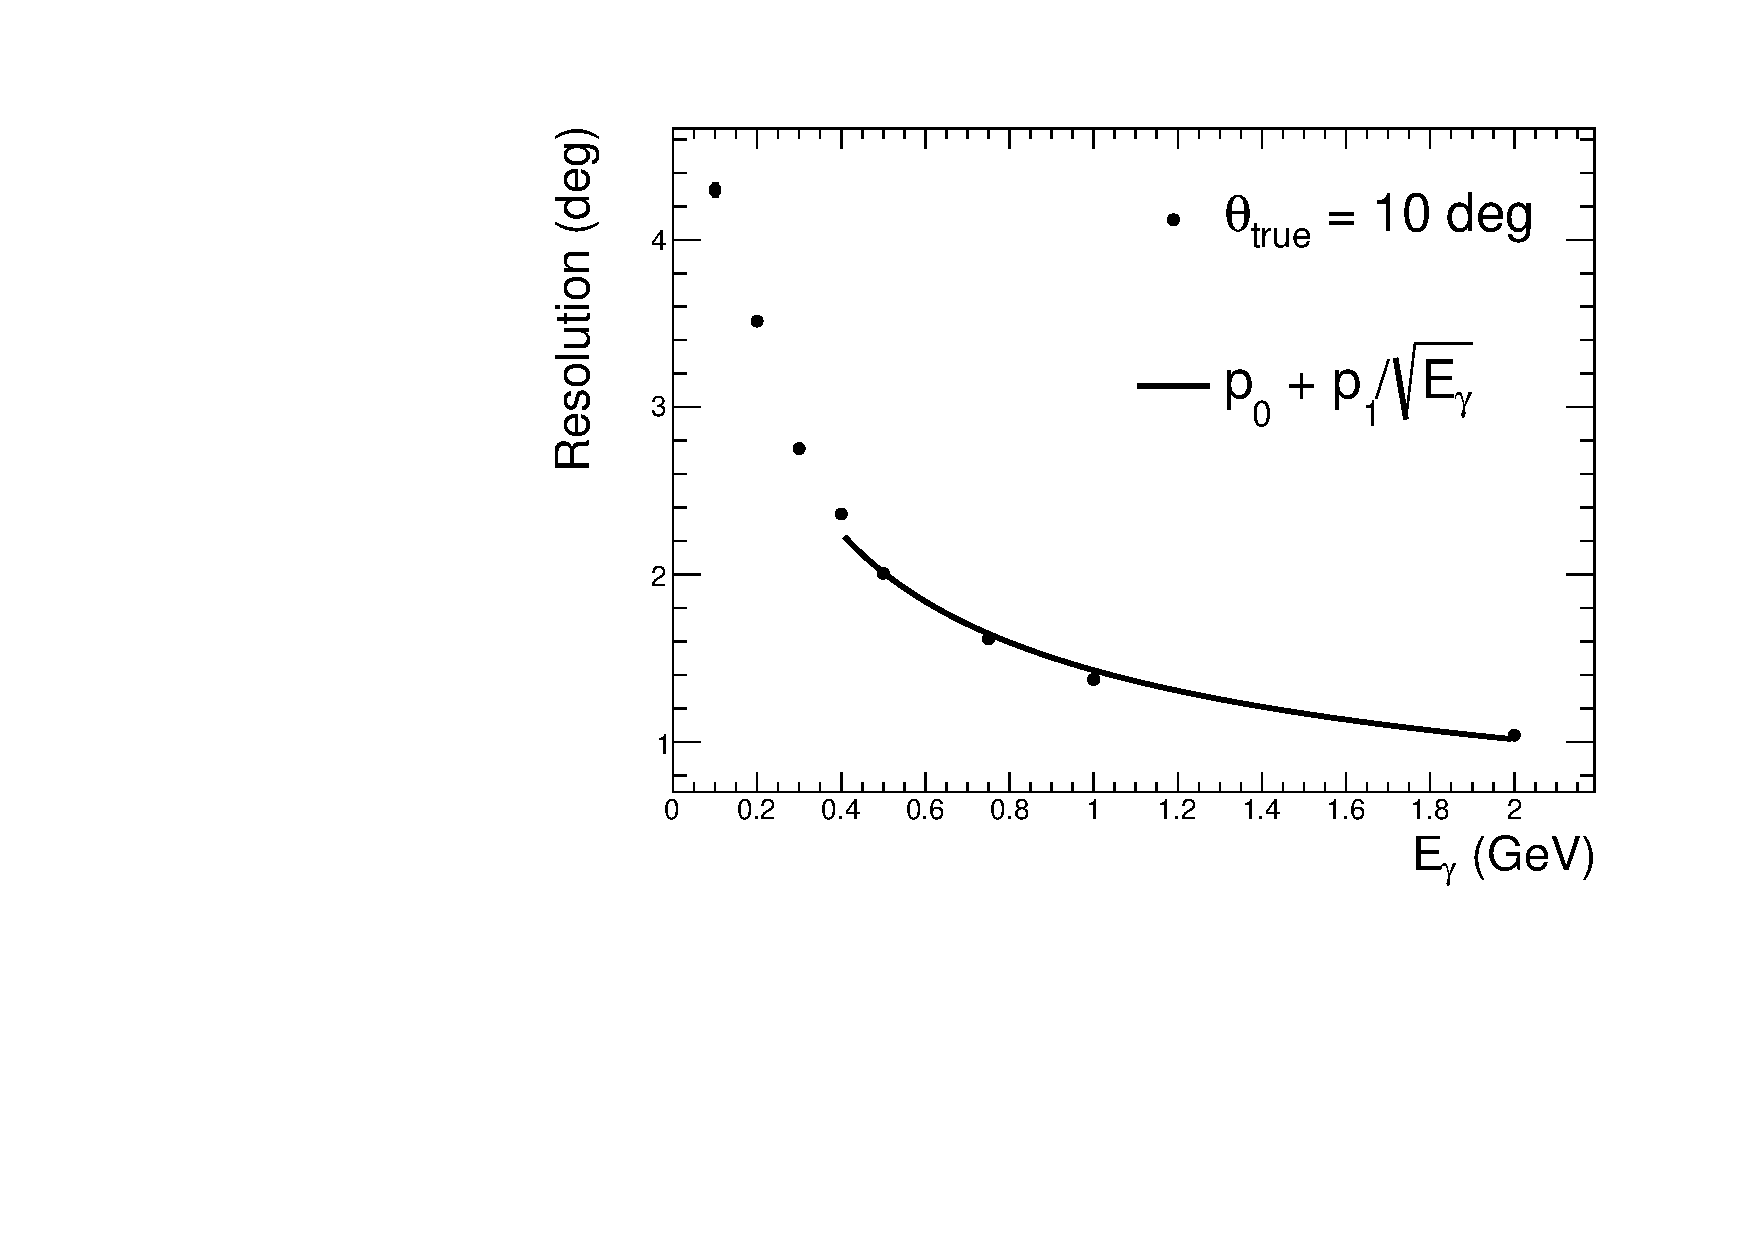
\includegraphics[width=0.48\textwidth]{figures/Fig5_reco_graph.pdf}
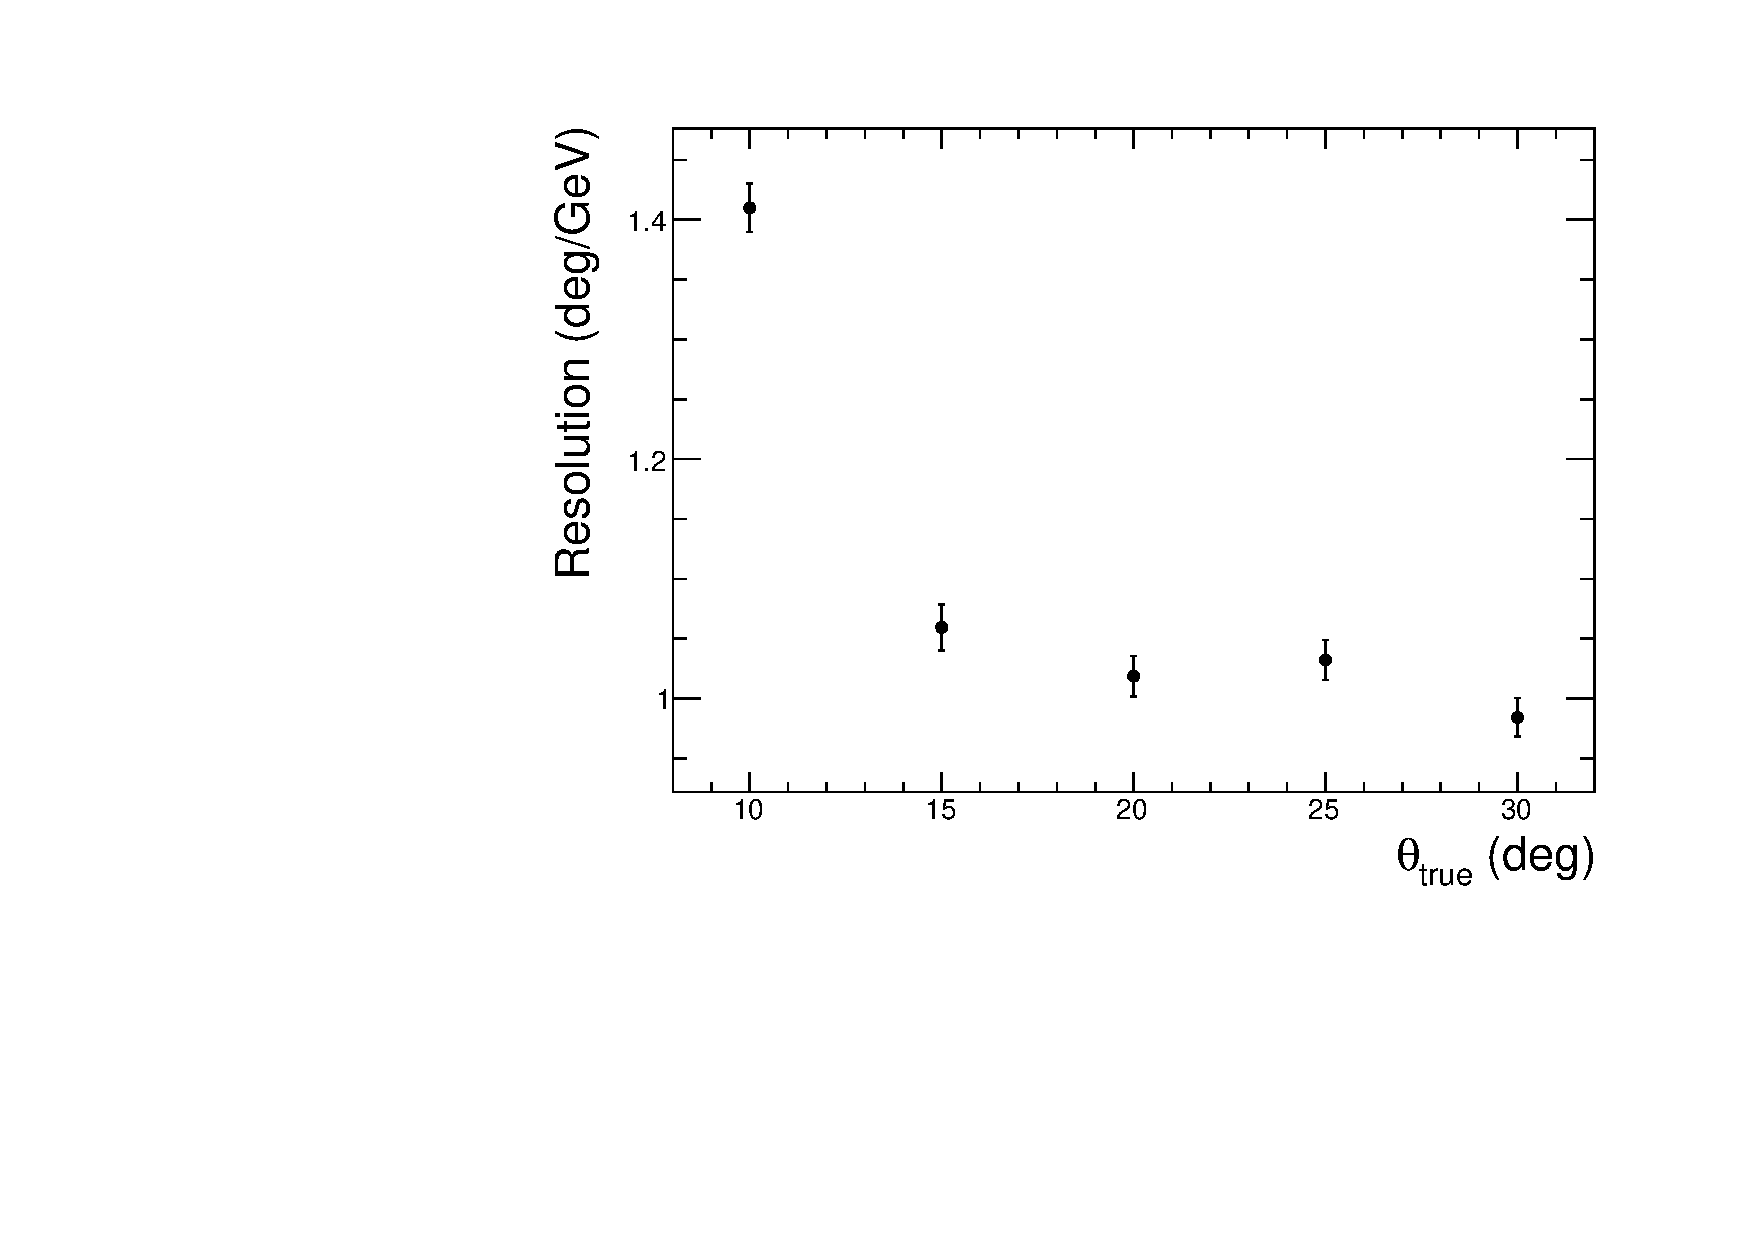
\includegraphics[width=0.48\textwidth]{figures/Fig5_reco_inc.pdf}
\caption{ The angular resolution as a function of the $\gamma$ energy (left), and $p_{1}$ for 1 GeV as a function of the incident angle (right). $p_{1}$ is consistent down to $\theta=$~15~deg and changing at $\theta=$~10~deg, which is coming from the definition of $\theta$ }
\label{fig:angle_reco_dep_gr}
\end{figure}

Figure~\ref{fig:angle_reco_dep_gr} shows the angular resolution as a function of the incident $\gamma$ energy for $\theta=$~10~degrees on the left panel. The resolution is fitted with $p_{0} + p_{1}/\sqrt{E_{\gamma}(GeV)}$, where the $p_{0}$ denotes the energy-independent contribution and is estimated to be 0.2, and the $p_{1}$ denotes the energy-dependent contribution, mainly related with the development of the EM shower. The estimated $p_{1}$ for different $\theta$ can be seen on the right panel of fig.~\ref{fig:angle_reco_dep_gr}. They are deviating within $\pm$~0.05~deg range from the 1.1~deg.

\begin{figure}[!hbt]
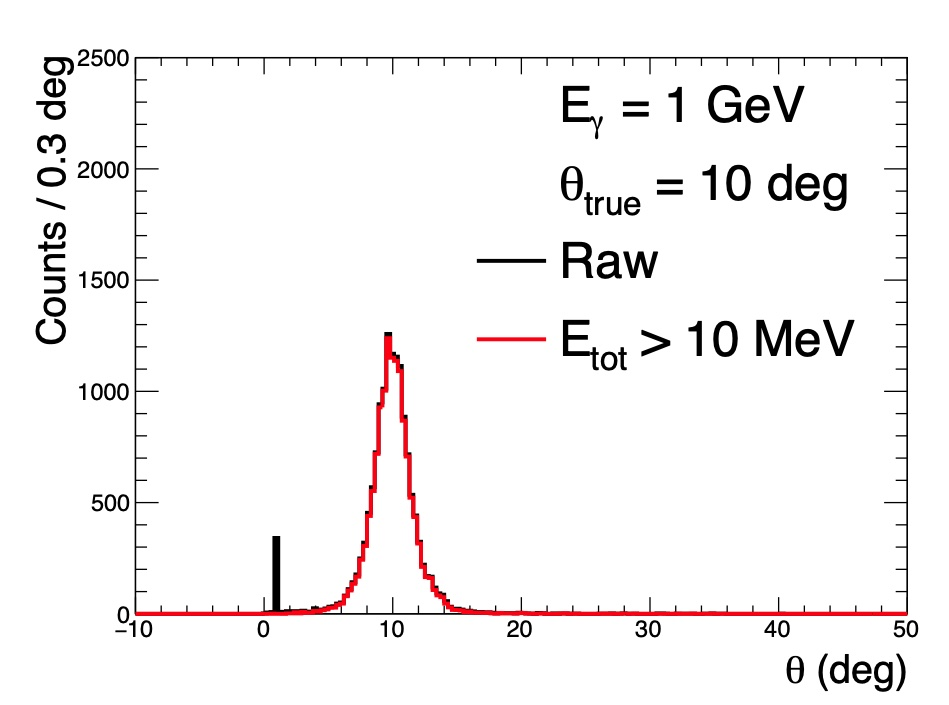
\includegraphics[width=0.48\textwidth]{figures/res_Nlayer.jpg}
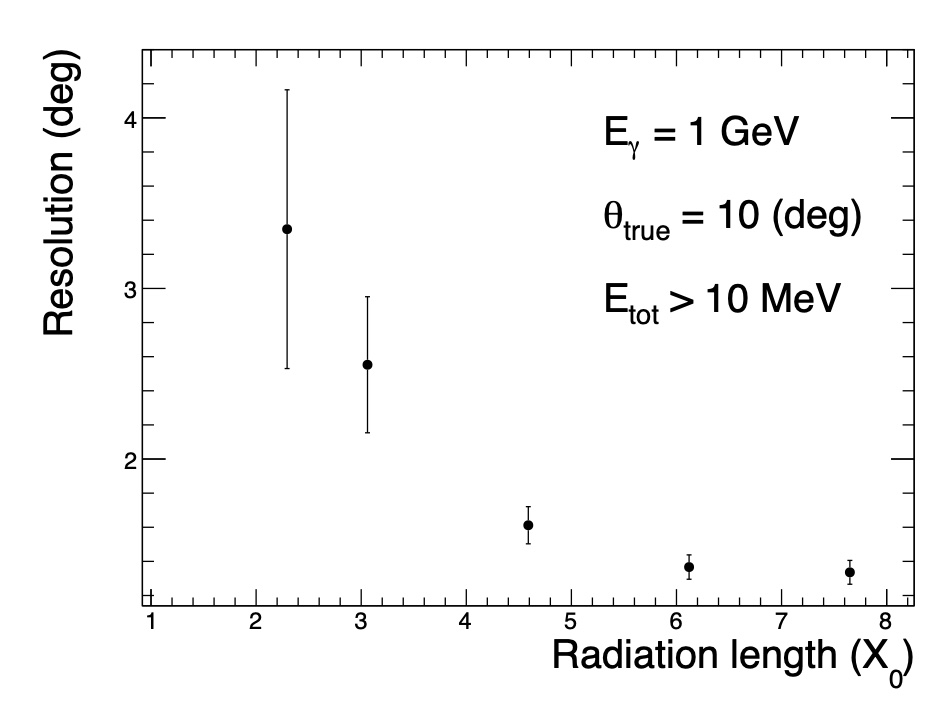
\includegraphics[width=0.48\textwidth]{figures/resol_Nlayer.jpg}
\caption{ Reconstructed $\theta$ for 1 GeV $\gamma$ with $\theta=$~10~deg with (red) and without (black) the total energy ($E_{\rm{tot}}$) selection (left), and the angular resolution as a function of front layer depth used for the reconstruction (right). The inefficiency for 4.6$X_{0}$ is estimated to be 5.8\% with 10~MeV selection. The large error bars less than 4.6$X_{0}$ is due to insufficient fitting because the reconstructed angular distributions deviated from the General Gaussian function.}
\label{fig:angle_reco_layer}
\end{figure}

The reconstruction of the incident angle is tested with the front layer instead of the full layers considering the cost-effectiveness from the fact that 99\% of the $\gamma$ generates the EM shower in front of 5$X_{0}$. The left panel of Figure~\ref{fig:angle_reco_layer} shows reconstructed angle using the front 24 layers of the detector, which corresponds to the 4.6$X_{0}$ for 1~GeV $\gamma$. Some $\gamma$s are failed to be reconstructed due to the lack of the channel having the energy deposit. The failed events are represented as a delta function near 0, and such events are removed by requiring the total energy deposit to be larger than 10~MeV. The angular resolution with the front layer is estimated to be XXX while possessing inefficiency estimated to be 5.8\%.

\begin{figure}[!hbt]
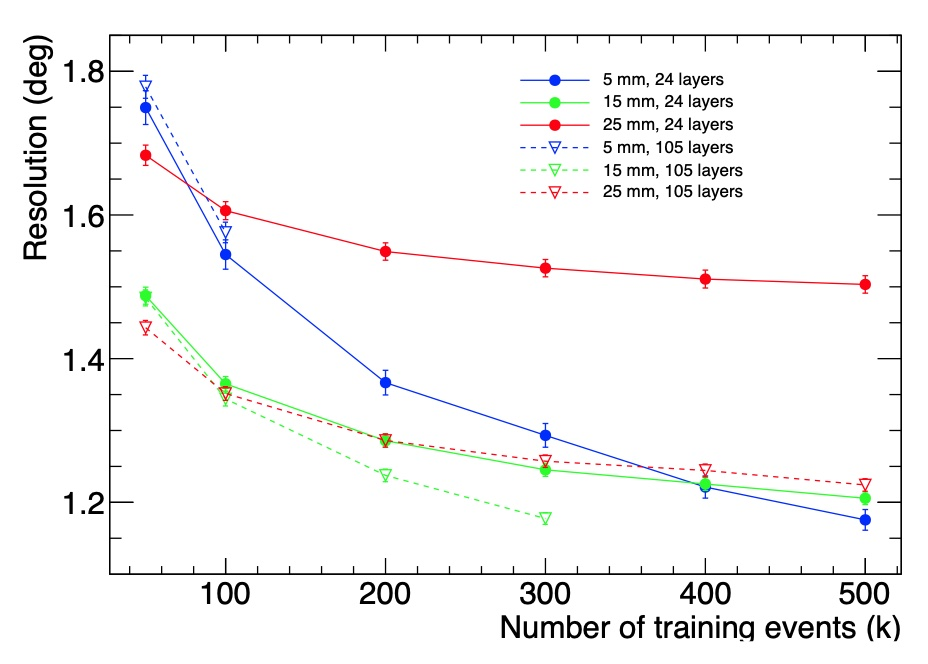
\includegraphics[width=0.6\textwidth]{figures/layer-event.jpg}
\caption{ The angular resolution for 1 GeV $\gamma$ with $\theta=$~10~deg as a function of the number of training samples with different strip widths using the first 24 layers or the full layers. }
\label{fig:multi-parameter}
\end{figure}

Figure~\ref{fig:multi-parameter} shows the angular resolution with different numbers of training samples for different detector configurations. All configurations show a decrease in the angular resolution with increasing training samples, which means that enhanced statistics for the training results in better reconstruction. The angular resolution with 5-mm-wide scintillator strips is more rapidly decreasing than others. The number of features for the 5-mm-wide strip is much larger than others, and the number of training samples is much required to correlate larger features. Considering limited computing resources, The setup with 2$\times10^{5}$ events, 24 layers, and the 15-mm-wide strip is chosen for the training of the $\XGB$, where the result is under 0.1 degree difference from the best setup.
 
\section{SUMMARY}
\label{sec:sum}

We conduct a feasibility study to measure the incident angle of the $\gamma$ with the finely segmented sampling calorimeter. With alternating 1-mm-thick lead plates and 5-mm-thick plastic scintillator strips, the EM shower is largely generated in lead sheets, and is measured by scintillators. The incident angle the $\gamma$ is reconstructed with the $\XGB$ using the energy deposited in each scintillator strip.

We optimize the hyperparameter of the $\XGB$, and optimize the detector configuration using the optimized $\XGB$. We scan the hyperparameter in the 5-dimensional space and find the set providing the best angular resolution for different detector configurations. We find that 15-mm-wide strips provide the best angular resolution, which can be expressed as 0.2+1.1$/ \sqrt{E_\gamma}$ for different incident angles. We also find that using 24 front layers gives the angular resolution which is compatible with the angular resolution we get from the full layer.

The angular resolution is changing with the variation of the training of the $\XGB$ and the detector configuration. As the strip width decreases, more channels of scintillator strips are required, and the training of the $\XGB$ gets affected due to the increased feature size. This is quenched with the larger number of training samples, which qualitatively improves the training of the $\XGB$. On the other hand, the longer strip width provides the worse angular resolution as the position resolution of the EM shower gets worse. We conclude that 15-mm-wide strips provide the favorable angular resolution with 24 front layers and 2$\times10^{5}$ training samples.

\label{sec:con}


%\pagebreak

\begin{acknowledgments}
\end{acknowledgments}

\bibliography{paper}

\end{document}
